\documentclass{article}

\usepackage{report/context/arxiv}

\usepackage[utf8]{inputenc} % allow utf-8 input
\usepackage{amsmath}
\usepackage[T1]{fontenc}    % use 8-bit T1 fonts
\usepackage{hyperref}       % hyperlinks
\usepackage{url}            % simple URL typesetting
\usepackage{booktabs}       % professional-quality tables
\usepackage{amsfonts}       % blackboard math symbols
% \usepackage{nicefrac}       % compact symbols for 1/2, etc.
% \usepackage{microtype}      % microtypography
% \usepackage{lipsum}		% Can be removed after putting your text content
\usepackage{graphicx}
\usepackage{natbib}
% \usepackage{doi}
\usepackage{float}
\usepackage{subcaption}
% \usepackage{wrapfig}



\title{[TITLE]}


\author{ \href{https://orcid.org/0000-0000-0000-0000}{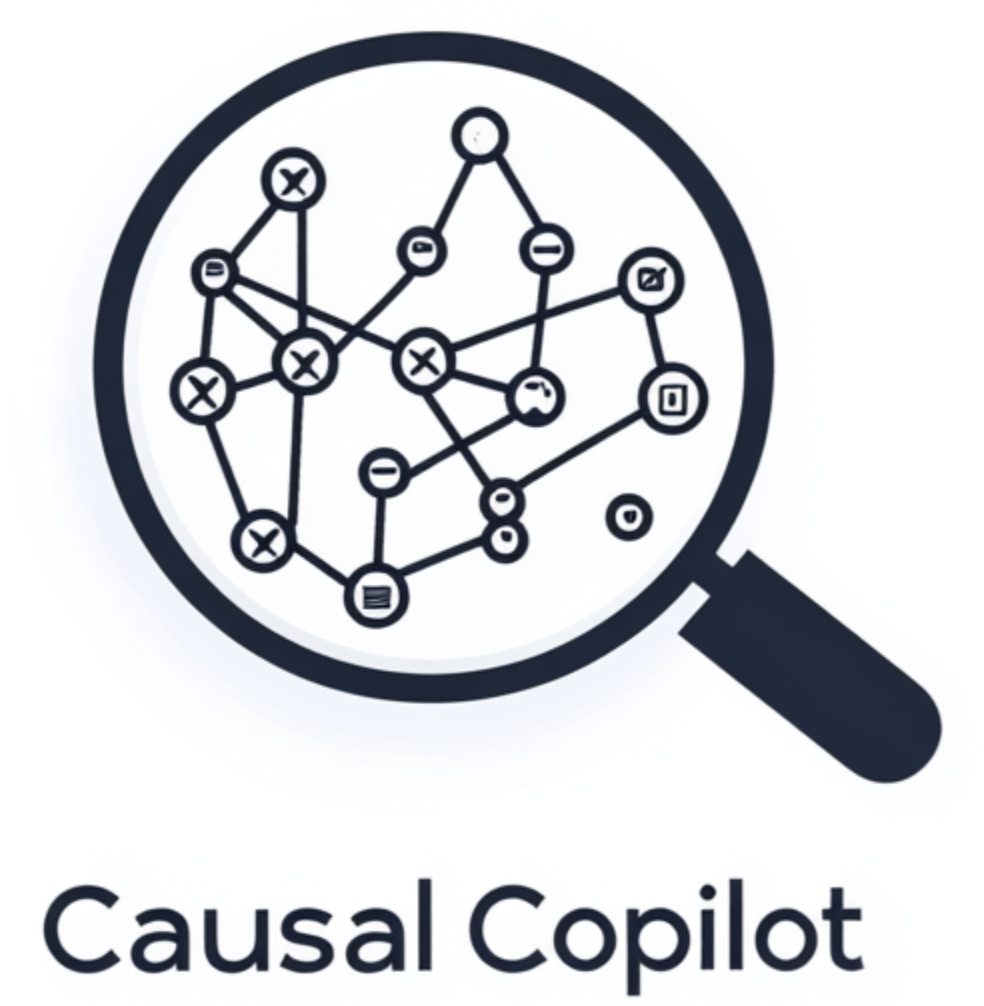
\includegraphics[scale=0.06]{asset/logo.png}} }
	

\renewcommand{\headeright}{Technical Report}
\renewcommand{\undertitle}{Technical Report}

\hypersetup{
pdftitle={[TITLE]},
pdfauthor={Causal Copilot},
pdfkeywords={Causal Discovery, Large Language Model, [ALGO], [DATASET]},
}

\begin{document}
\maketitle

\begin{abstract}
[ABSTRACT]
\end{abstract}

\keywords{Causal Discovery, Large Language Model, [ALGO], [DATASET]}

\raggedbottom
\section{Introduction}
[INTRO_INFO]

\section{Background Knowledge}
\subsection{Detailed Explanation about the Variables}
[BACKGROUND_INFO1]

\subsection{Possible Causal Relations found by LLM}

The following are potential causal relationships suggested by the language model, which are visualized in Figure 1. Please note that only variables present in our dataset are included in the figure.

[BACKGROUND_INFO2]

\section{Dataset Descriptions and EDA}
The following provides a preview of our original dataset. If the dataset contains more than 10 columns, a random subset of 10 columns is displayed for illustrative purposes.

\begin{table}[H]
    \centering
    \caption{Dataset Preview}
    [DATA_PREVIEW]
\end{table}

\subsection{Data Properties}

We employed several statistical methods to identify data properties, including:

\textbf{Basic Data Characteristics}

The shape of the data, variable types, and the presence of missing values were assessed directly from the DataFrame. 
In contrast, properties such as time-series structure and heterogeneity were inferred with LLM based on user queries and DataFrame.

\textbf{Linearity Testing}

We conducted the Ramsey's RESET test to assess linearity between each pair of variables. When the total number of possible variable pairs was fewer than 100, all pairs were tested. If the number exceeded 100, a random subset of 100 pairs was selected for testing to ensure computational feasibility. 
To account for multiple testing, we employed the Benjamini and Yekutieli procedure, which is robust when dealing with dependent or correlated data. 
The linearity assumption was considered satisfied only if all tested pairs exhibited linearity; otherwise, it was considered violated.

\textbf{Normality of Residuals}

The assumption of Gaussian (normally distributed) noise was assessed using the Shapiro-Wilk test. 
The testing approach depended on the outcome of the linearity evaluation. 
If linearity was satisfied, we fitted ordinary least squares (OLS) models for each variable pair and extracted the residuals for testing. 
If linearity was not satisfied, we used a flexible non-parametric method—locally weighted scatterplot smoothing (LOWESS)—to model the relationships and obtain residuals. 
The Benjamini and Yekutieli correction was again applied to control for false discovery under multiple testing.


[PREPROCESS_GRAPH]

Properties of the dataset we analyzed are listed below.

\begin{table}[H]
    \centering
    \caption{Data Properties}
[DATA_PROP_TABLE]
\end{table}

[EDA_INFO]

\section{Causal Discovery Procedure}
[DISCOVER_PROCESS]

[CAUSAL_GRAPH]

[RESULT_ANALYSIS]

\clearpage

\subsection{Revised Graph}

\subsubsection{Bootstrap Probability}
[CONFIDENCE_GRAPH]

[RELIABILITY_ANALYSIS]

\subsubsection{LLM Pruning}

[REVISE_PROCESS]


\subsection{Graph Reliability Analysis}

[REFUTATION_GRAPH]

[RESULT_GRAPH_COMPARISION]
[RESULT_COMPARISION]

\subsection{Conclusion}
[CONCLUSION]

[INFERENCE]

\end{document}
